\clearpage
\section{保存浴室后，已烘焙的反光回到了实时更新}

浴室里有镜前、窗边和门边三盏点光源。互换两盏灯在场景文件中出现的位置，房间实际收到的光仍然一样。可是旧版编辑器在烘焙成功后，只要按 Ctrl+S、退出、重新打开同一场景，面板就会提示重新烘焙。直接退出再打开原来的文件，却能沿用旧结果。

\begin{figure}[H]\centering
\begin{minipage}[b]{.48\linewidth}\centering
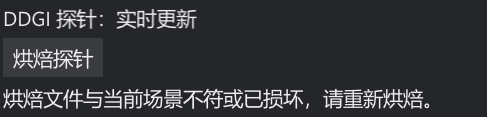
\includegraphics[width=\linewidth]{../../../output/validation/probe-order/before.png}\\{\small 旧版本重开，提示重新烘焙}
\end{minipage}\hfill
\begin{minipage}[b]{.48\linewidth}\centering

\includegraphics[width=\linewidth]{../../../output/validation/probe-order/after.png}\\{\small 修正后重开，沿用已保存的探针}
\end{minipage}
\caption{两次都先在正式编辑器内烘焙，再保存、退出并重开浴室。左图从旧版窗口截图裁取，右图从新版 RenderDoc 第 12 帧的编辑器画面裁取。}
\end{figure}

将保存前后的 YAML 并排查看，五个实体从 $4,3,2,5,1$ 变为 $1,5,2,3,4$。灯的位置与强度都没动。旧的 \texttt{ProbeKey} 把整个灯数组当成一串字节，顺着它们在文件中的排列计算校验值。两盏灯互换位置以后，读到的字节顺序已经不同，于是程序拒绝了本来还能用的文件。

\noindent{\small C++，\path{Renderer/GI/GlobalIllumination.cpp}。以下是修正前的返回语句，其中 \texttt{key} 已包含几何与取样种子。}
\begin{Code}
// 按数组先后读取各盏灯；另存为时这个顺序可能改变。
return ProbeBake::Hash(key, Lights.data(), Lights.size() * sizeof(GILight));
\end{Code}

现在先分别给每盏灯的位置、颜色与强度算一个值，再按从小到大合并这些值。三盏灯写入文件的先后就不影响结果。多个模型也按场景中固定的实体编号建碰撞树，因为树里三角形的排列同样会进入校验。这个顺序只用来认出同一间房。真的挪走窗边灯或换掉一面墙时，程序仍会要求重新烘焙。

修正后用两个独立进程再次打开浴室，面板保持「已烘焙」。RenderDoc 第 12 帧有 8 次计算调度，省去了更新探针的一次。独立回归另外交换两盏灯的顺序，并颠倒两个不同颜色和位置的模型；两次都能读回原文件。改灯强或替换几何时，两次都拒绝使用旧文件。\href{run:../../output/validation/probe-order/reproduction.json}{两次实拍记录}\quad\href{run:../../tests/ProbeBakeCheck.h}{C++ 回归用例}
